%%%%%%%%%%%%%%%%%%%%%%%%%
%                       %
% Luther Michaels       % 
% ECE 351-52            %
% Lab 10                %
% November 11, 2021     %
% Frequency Response    %
%         Lab Report    %
%                       %
%%%%%%%%%%%%%%%%%%%%%%%%%

%%%%%%%%%%%%%%%%%%%%%%%%%%%%%%%%%%%%%%%%%%%
%%% DOCUMENT PREAMBLE %%%
\documentclass[12pt]{report}
\usepackage[english]{babel}
\usepackage{url}
\usepackage[utf8x]{inputenc}
\usepackage{amsmath}
\usepackage{graphicx}
\graphicspath{{images/}}
\usepackage{parskip}
\usepackage{fancyhdr}
\usepackage{vmargin}
\usepackage{listings}
\usepackage{hyperref}
\usepackage{xcolor}
\usepackage{caption}

\newcommand{\adjust}{\hspace{2em}}

\definecolor{codegreen}{rgb}{0,0.6,0}
\definecolor{codegray}{rgb}{0.5,0.5,0.5}
\definecolor{codeblue}{rgb}{0,0,0.95}
\definecolor{backcolour}{rgb}{0.95,0.95,0.92}

\lstdefinestyle{mystyle}{
	backgroundcolor=\color{backcolour},   
	commentstyle=\color{codegreen},
	keywordstyle=\color{codeblue},
	numberstyle=\tiny\color{codegray},
	stringstyle=\color{codegreen},
	basicstyle=\ttfamily\footnotesize,
	breakatwhitespace=false,         
	breaklines=true,                 
	captionpos=b,                    
	keepspaces=true,                 
	numbers=left,                    
	numbersep=5pt,                  
	showspaces=false,                
	showstringspaces=false,
	showtabs=false,                  
	tabsize=2
}

\lstset{style=mystyle}

\setmarginsrb{3 cm}{2.5 cm}{3 cm}{2.5 cm}{1 cm}{1.5 cm}{1 cm}{1.5 cm}

\title{10}	% Title						
\author{Luther Michaels}	% Author		
\date{November 11, 2021}   % Date

\makeatletter
\let\thetitle\@title
\let\theauthor\@author
\let\thedate\@date
\makeatother

\pagestyle{fancy}
\fancyhf{}
\rhead{\theauthor}
\lhead{\thetitle}
\cfoot{\thepage}
%%%%%%%%%%%%%%%%%%%%%%%%%%%%%%%%%%%%%%%%%%%%

\begin{document}
	
%%%%%%%%%%%%%%%%%%%%%%%%%%%%%%%%%%%%%%%%%%%%%%%%%%%%%%%%%%%%%%%%%%%%%%%%%%%%%%%%%%
%%% TITLE PAGE %%%
\begin{titlepage}
	\centering
	\vspace*{0.5 cm}
		
	\begin{center}    
		\textsc{\Large   ECE 351 - Section \#52}\\[2.0 cm]	
	\end{center}  
	\textsc{\Large Frequency Response  }\\[0.5 cm]
	\rule{\linewidth}{0.2 mm} \\[0.4 cm]
	{ \huge \bfseries \thetitle}\\
	\rule{\linewidth}{0.2 mm} \\[1.5 cm]
	\begin{minipage}{0.4\textwidth}
		\begin{flushleft} \large
		\end{flushleft}
	\end{minipage}~
	\begin{minipage}{0.4\textwidth}
		\begin{flushright} \large
			\emph{Submitted By:} \\
			Luther Michaels \break
			
			\emph{Submission Date:} \\
			November 11, 2021
		\end{flushright}
	\end{minipage}\\[2 cm]
\end{titlepage}
	
%%%%%%%%%%%%%%%%%%%%%%%%%%%%%%%%%%%%%%%%%%%%%%%%%%%%%%%%%%%%%%%%%%%%%%%%%%%%%%%%%%
%%% TABLE OF CONTENTS %%%

\tableofcontents
\pagebreak

%%%%%%%%%%%%%%%%%%%%%%%%%%%%%%%%%%%%%%%%%%%%%%%%%%%%%%%%%%%%%%%%%%%%%%%%%%%%%%%%%%
%%% LAB REPORT %%%
\renewcommand{\thesection}{\arabic{section}}
\section{Introduction}
		  
The central focus of this lab is on analysis of frequency response using Bode plots. The goal is to study a filter through the construction of a Bode plot from its transfer function using several methods in Python. The knowledge accrued about this filter can then be utilized to observe its effects on a sinusoidal input function. \\

Several new Python functions will be essential in properly completing this procedure. The numpy package functions numpy.arctan() and numpy.log10() will be needed to implement the magnitude in decibels and phase of the transfer function. The former function notably returns a value in radians. A plot axis may be formatted on a logarithmic scale with matplotlib.pyplot.semilogx(). The magnitude and phase of a transfer function can be found using the scipy package function scipy.signal.bode(). A transfer function can be formatted for the control package with control.TransferFunction() and its Bode plot created in Hertz with control.bode(). The digital form of a filter can be determined with scipy.signal.bilinear() by transforming its components into the z-domain. The result of an input attenuated by a digital filter can be found with scipy.signal.lfilter(). All output and plots can be produced through Python implementation written within the Spyder software. \\

\section{Equations}

\begin{equation}
	H(s) = \frac{\frac{1}{RC}s}{s^2 + \frac{1}{RC}s + \frac{1}{LC}}
\end{equation}
\begin{equation}
	|H(j\omega)| = \frac{\frac{1}{RC}\omega}{\sqrt{\omega^4 + \omega^2(\frac{1}{R^2C^2} - \frac{2}{LC}) + \frac{1}{L^2C^2}}}
\end{equation}
\begin{equation}
	\angle H(jw) = 90^\circ - tan^{-1}(\frac{\frac{1}{RC}\omega}{-\omega^2 + \frac{1}{LC}})
\end{equation}
\begin{equation}
	dB = 20\cdot log_{10}(|H(j\omega)|)
\end{equation}
\begin{equation}
	x(t) = cos(2\pi\cdot 100t) + cos(2\pi\cdot 3024t) + sin(2\pi\cdot 50000t)
\end{equation}
\begin{equation}
	\omega = 2\pi f
\end{equation}

\section{Methodology}

The first task of Part 1 requested plots be created for the magnitude and phase derivations found in the prelab from the transfer function in Equation 1. The step size was given as $ 10^{-1} $ in order to allow for both good resolution and practical timing. The frequency in $ \frac{rad}{sec} $ was initialized over the interval from $ 10^3 $ to $ 10^6 $ using numpy.arange. Separate functions were written to implement Equations 2 and 3 with the frequency and filter characteristics as parameters. In using the package command numpy.arctan() to model the equation, the output had to first be translated to degrees using the conversion factor $ \frac{180^\circ}{\pi} $. \\

After calling both functions with the specified filter values, the magnitude was converted to decibels using Equation 4 and the function numpy.log10(). The magnitude and phase were plotted on a logarithmic scale using matplotlib.pyplot.semilogx() in place of the regular plot instruction. Apart from this change, the standard sequence of matplotlib.pyplot commands from prior labs were used to organize the graph as a single figure with two subplots. \\ 

In Task 2 of Part 1, these two plots were to be verified using the Python package function scipy.signal.bode(). This was accomplished by first writing a function to represent Equation 1. The filter characteristics were passed to the function, while matrices for the numerator and denominator were returned. Once the function was called, these matrices were passed to the scipy bode function alongside the frequency variable to obtain the magnitude in decibels and the phase. Each was then plotted as in the prior task and compared with their counterpart. \\

The resultant plot of the phase in Task 2 revealed that an adjustment would be required to obtain an accurate result for the phase in Task 1. The function for Equation 3 was altered to include a loop that iterated through each value of the phase while checking for values greater than $ 90^\circ $. Any points that satisfied this conditional would have their value reduced by $ 180^\circ $. Consequently, the right-hand portion of the phase plot would be lowered to form a cohesive shape. \\

The third task of Part 1 was to create a bode plot for the transfer function across a frequency spectrum measured in Hertz using the Python control package. The numerator and denominator defined previously were provided to the function control.TransferFunction() to arrange the system for further use. Following the sample code in the lab manual, this system was utilized by control.bode() with the proper settings to produce the desired plot. A title was attempted to be given to the graph, but it would not display properly above the plot. As a result, the title included in the Results section of this report was written as a figure caption. \\ 

In Part 2 of the procedure, the first task was to plot Equation 5 over the time interval from $ 0 $ to $ 0.01 $ seconds. A sampling frequency of $ 10^5 $ was chosen to properly display the signal, and the step size was defined to be its reciprocal. The time variable was assigned with numpy.arange() and this new step size. The equation was then assigned to a variable and plotted using the standard process as before. \\

Tasks 2 and 3 of Part 2 required that the transfer function be converted into the z-domain such that the input signal could then be filtered using the results of this transformation. The z-domain form was acquired using scipy.signal.bilinear() with inputs of the transfer function matrices and the sampling frequency. The numerator and denominator returned were then passed to the function scipy.signal.lfilter() alongside Equation 5 to identify the filtered output. The fourth task of Part 2 was to plot the filtered signal obtained in the prior task. This was done using the same sequence of matplotlib.pyplot commands to arrange and label the plot. The x-axis was matched to that of the plot in Task 1 of Part 2 by employing the same time variable. \\

Github Link: \url{https://github.com/Luther-Michaels} \\

\section{Results}

With the completion of two functions implementing the magnitude and phase derivations, the bode plot of the transfer function in Equation 1 was obtained as shown below. The subplots are arranged in typical bode fashion with the magnitude in decibels above the phase. While the time required to produce the graph is minimal, the step size is still sufficiently small to display with good resolution. The x-axis demonstrates that the frequency interval has been set between $ 10^3 $ and $ 10^6 $ $ \frac{rad}{sec} $. \\

The starting behavior of both subplots matches our expectation given the s factor in the numerator of Equation 1. The magnitude initially increases with the s, begins to briefly flatten, and eventually decreases as prescribed by the imaginary poles in the denominator. It also moves between decades at a rate of 20 dB per decade as our intuition suggests. The overall shape of the magnitude is supported by the realization that the general form of the transfer function can be identified as a bandpass filter. The plot clearly shows minimal attenuation only at middle frequencies as we would expect. The phase decreases from $ 90^\circ $ to $ -90^\circ $ across the entire interval. Given the non-real poles, this trend can best be verified by the subsequent scipy plot. \\

\begin{center}
	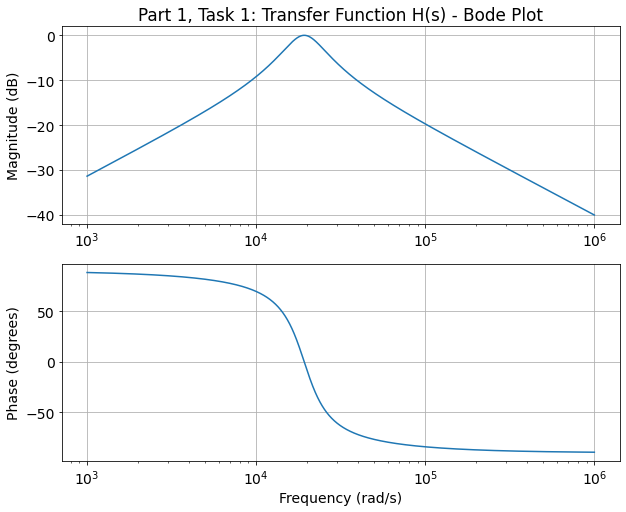
\includegraphics[scale = 0.38]{Lab 10 - Plots/Part1-Task1.png}\\[0.5 cm]
\end{center}

The bode plot shown below was created using the Python scipy package bode function to obtain the magnitude and phase components. The subplots are identical to their counterparts in the prior graph. The shapes and their axes move across the same intervals. This serves to support the results of the plot obtained in the first task. Specifically, the plot of the phase shows that the adjustments made to the phase function in Python were appropriate. The right half of the signal is lower such that the total y-axis displacement is $ 180^\circ $. \\

\begin{center}
	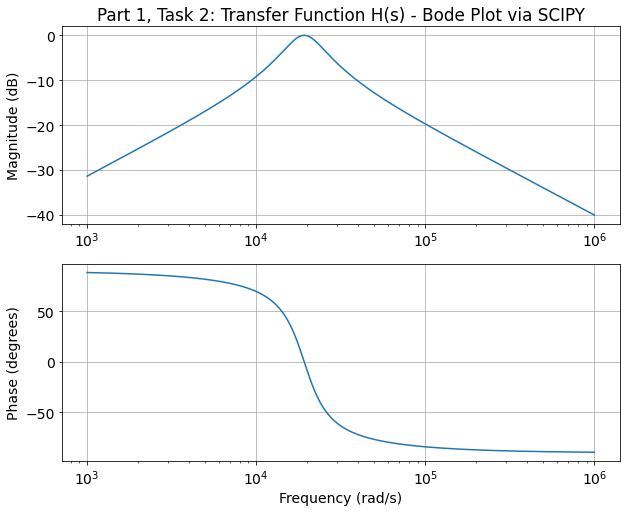
\includegraphics[scale = 0.38]{Lab 10 - Plots/Part1-Task2.png}\\[1.0 cm]
\end{center}

The next graph shows the bode plot conversion for the frequency range given in Hertz. The shapes of the magnitude and phase have been preserved as well as the y-axis of the upper subplot. The change in frequency unit has altered the y-axis of the phase. This makes sense given the relationship between the two units for frequency described by Equation 6. The original values have all been subtracted by $ 2\pi $ or $ 360^\circ $. Due to the use of the control function, the title of this plot could not be produced in Python, but was rather implemented as a caption in this report. \\

\begin{figure}[h]
	\begin{center}
		\caption*{\scriptsize \adjust Part 1, Task 3: Bode Plot in Hertz}
		\vspace*{-0.43 cm}
		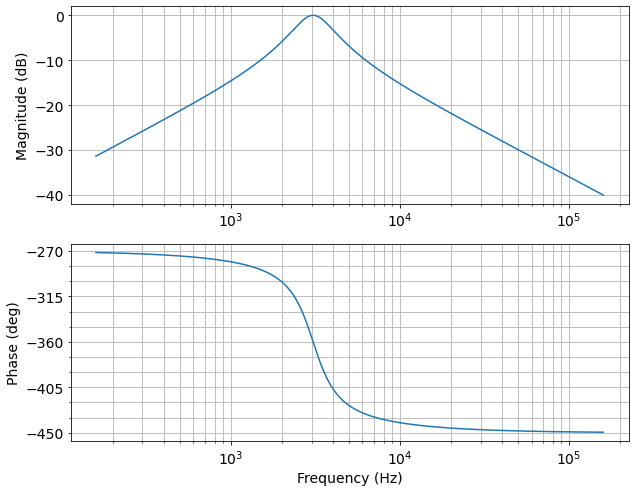
\includegraphics[scale = 0.5]{Lab 10 - Plots/Part1-Task3.png}\\[0.3 cm]
	\end{center}
\end{figure}

The following figure shows the time-domain plot of Equation 5 impacted by its three distinct sinusoidal functions. As one would expect, the general shape is sinusoidal and upon closer inspection reveals three different frequencies. This indicates that the sampling frequency and associated step size have been adequately selected. The time interval is properly set from $ 0 $ to $ 0.01 $ seconds as requested. The period of each term is $ 1 $ second and the initial value is $ 2 $. This initial value makes sense given the equation is composed of two cosine functions with values of $ 1 $ for an input of $ 0 $. \\

\begin{center}
	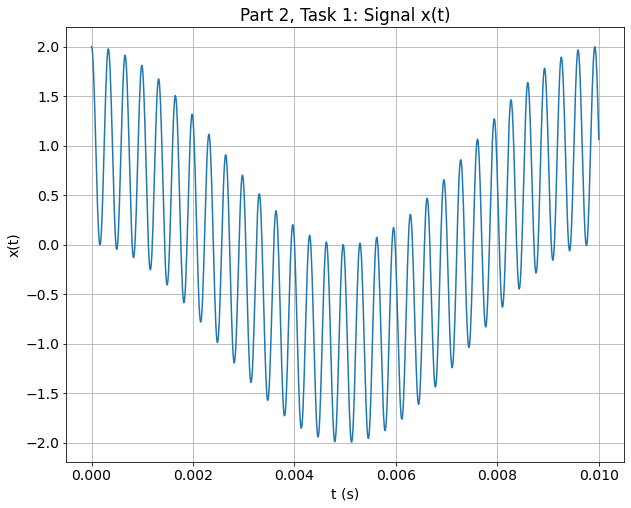
\includegraphics[scale = 0.4]{Lab 10 - Plots/Part2-Task1.png}\\[0.4 cm]
\end{center}

The final plot displays the altered result of Equation 5 when run through the filter described by the transfer function in Equation 1. The x-axis time scale is shown to cover the same interval as the prior plot. As the middle cosine is the only sinusoidal function within the equation that has a frequency which falls between the filter's cutoff frequencies shown in the prior bode plots, one would expect its values to receive almost no attenuation. Consequently, the middle term is the major contributor to the result and can be looked to in order to analyze the plot. This is supported by the new maximum amplitude of about $ 1 $, since there is only one cosine principally in play. Additionally, the final plot shows a single consistent frequency as opposed to the three original. The sinusoidal shifting amplitude has been dramatically reduced. \\

\begin{center}
	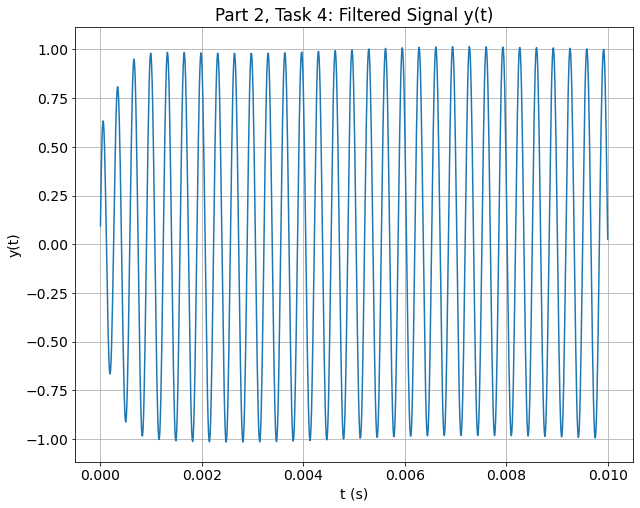
\includegraphics[scale = 0.4]{Lab 10 - Plots/Part2-Task4.png}\\[1.0 cm]
\end{center}

\section{Error Analysis}

I initially struggled to match the phase plot in Task 1 to that found with scipy in Task 2. After consulting the TA, I was informed that the numpy.arctan() function would return a result in radians which must be converted to degrees. This was done using the conversion factor $ \frac{180^\circ}{\pi} $. With this change, I was able to determine a fix for my phase iteration adjustment and produce an identical image to its counterpart. \\

I also had difficulty in understanding the input to scipy.signal.bilinear() at first. I would receive an error saying that the output was too great. With the help of the TA once again, I realized that I was trying to input the numerator and denominator of Equation 5 rather than the filter components. This correction allowed the filter output to respond as expected. \\

I could not determine how to provide a title for my bode plot created with the control package. I first attempted to label it as with the other plots, but the title was either not included at all or placed in the center between the subplots. I also tried to implement it as an argument for the parameters defining matplotlib.pyplot options. Neither method worked and I had to place a caption directly into the report. \\ 

\section{Questions}

1. As discussed in the Results section, the filtered output in Part 2 makes sense given the Bode plots in Part 1 due to the predominance of a single cosine function with a frequency between the bandpass filter's two cutoff frequencies. The middle cosine term is seen to be contributing the most due to the amplitude change and the apparent single frequency across the entire shape. The filter modifies low and high frequency bands, attenuating increasingly outward. The middle frequencies around halfway between $ 10^3 $ and $ 10^4 $ Hz receive minimal attenuation. \\

2. The purpose of scipy.signal.bilinear() is to convert the filter numerator and denominator into the z-domain. According to its documentation, the function creates a digital representation of the filter by substituting $ \frac{z - 1}{z + 1} $ in for s. The outcome of scipy.signal.lfilter() is then the attenuated result of the input equation utilizing the z-domain filter components. This function is specifically designed to employ a digital filter to produce a filtered output of a given equation. \\

3. If a different sampling frequency is used in scipy.signal.bilinear() as opposed to what was used for the time-domain signal, the result is quite different. The plot shows an initial decaying sinusoidal shape with the impact of several different terms clearly still in play. A consistent frequency and amplitude is eventually reached, but the values do not match those achieved using the same sampling frequency for both scenarios. We can infer that the different sampling rates produce inaccurate results. \\

4. The lab tasks, expectations, and deliverables were all presented clearly. \\

\section{Conclusion}

In this lab we analyzed frequency response by building and observing Bode plots of filter transfer functions. We were introduced to a myriad of new Python functions including those in the control package. We were given a precursor to the concept of the z-domain and digital filters. This lab successfully presented a tangible, visual representation of the effects of filtering and helped bring the concepts to life. \\

If this lab were to be repeated, I would have the lab manual give an explanation of the two Python functions in Tasks 2 and 3 of Part 2. The z-domain will not have been covered in class lectures up to this point, and the functions' documentation pages are a little unclear on certain aspects of their operation. Through this lab, I necessarily learned to better research the documentation and develop understanding of the various Python functions we employ. The ability to determine how to use functions relating to known concepts independently will be of great help in understanding any future applications that may require new commands be introduced.

\newpage
\begin{thebibliography}{111}
	
	\bibitem{S}
	Sullivan, Dennis M. (2018) {\it  Signals and Systems for Electrical Engineers I}. Nevada: CreateSpace Independent Publishing Platform.
	
\end{thebibliography}
\end{document}

% Lab Report based on template created by Roza Aceska.